\section{基于帧间信息生成本底值}\label{sec:3}

由于钡餐浓度随时间变化大,且在不同器官中的形态变化大,难以从单帧图像中应用分割算法获得令人满意的结果。在\cref{sec:2} 中,我们完成了医学视频数据的预处理,包括窗口调整以及配准。接下来,我们主要尝试从视频序列带来的运动信息中提取关于钡餐的有效信息。

\subsection{逐帧求绝对差图像}

在本节中,我们针对视频数据进行处理,通过计算每一帧与其上一帧之间的差值,提取有意义的动态信息。具体来说,我们对视频中的每一组相邻帧进行逐一比较和相减。在求得差值后,我们对差值图像的每个像素点都取绝对值,从而得到一系列绝对差图像。对于运动中的物体,绝对差图像可以有效地显示出其轮廓。

\begin{figure}[!htp]
    \centering
    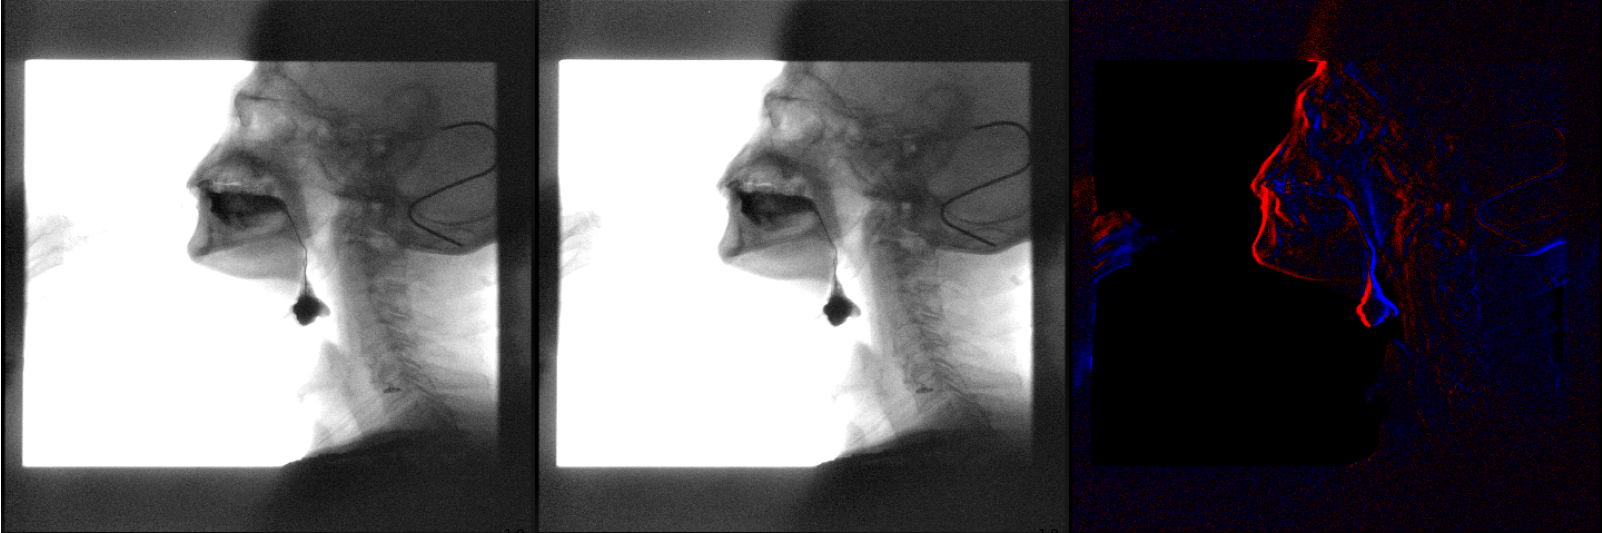
\includegraphics[width=\textwidth]{figures/3_1.png}
    \caption{相邻帧极其绝对差图像}
    \label{fig:3_2_绝对差}
\end{figure}

\subsection{图像噪点过滤}

由于吞咽钡餐时,受试者头部运动幅度显著,且配准技术无法将每一帧图像的每一个像素完全矫正准确,因此在求绝对差图像后,会出现噪点,需要进一步使用其它图像处理方法来去噪。本研究先使用双边滤波法进行初步降噪,随后循环使用形态学操作相关算法进行进一步去噪。

\subsubsection{双边滤波降噪}

双边滤波(Bilateral Filter,BF)是图像处理中的一种非线性滤波技术,该技术是对传统的高斯低通滤波器的优化。双边滤波在对图像数据进行处理时,充分考虑了像素之间的空间关系和像素值信息。这种滤波算法基于两个高斯函数组合而成,对目标像素的邻近区域像素进行灰度值的高斯加权计算,从而得到该像素点所需的像素值。其中,两个高斯函数分别负责处理空间接近程度的权重信息和灰度值相似性的权重信息。简单来说,如果一组临近像素点的灰度值相似,则双边滤波会对其进行平滑处理;反之,若临近像素点的灰度值差异大,则双边滤波不会对其进行处理,达到保持图像边缘的效果。当这两个函数共同作用时,双边滤波能够实现边缘保留和去噪的效果。

双边滤波过程的伪语言描述如下:

\begin{itemize}
    \item 输入: 待处理图像 $I$,空间高斯函数标准差 $SS$,范围高斯函数标准差 $SP$
    \item 输出:处理后图像 $J$
    \subitem 初始化 $J$ 为空
    \subitem 遍历 $I$ 的每个像素点 $(x, y)$:
    \subitem 初始化加权和 $weightSum$ 和 $normFactor$ 为 0
    \subitem 遍历像素 $(x, y)$ 周围的窗口大小为 $w$ 的邻域内的每个点 $(i, j)$:
    \subsubitem 计算空间高斯权值: $spatialWeight = G((x-i)^2 + (y-j)^2, SS)$
    \subsubitem 计算范围高斯权值: $rangeWeight = G((I(x,y) - I(i,j))^2, SP)$
    \subsubitem 计算双边权值: $bilateralWeight = spatialWeight \times rangeWeight$
    \subsubitem 更新加权和: $weightSum += I(i, j) \times bilateralWeight$
    \subsubitem 更新归一化因子: $normFactor += bilateralWeight$
    \subitem 求当前像素的滤波后值: $J(x, y) = \frac{weightSum}{normFactor}$
    \item 其中,高斯核函数 $G$ 是用来计算高斯值的函数。它的形式为:$G(x, \sigma) = e^{\frac{-x}{2\sigma^2}}$
\end{itemize}

\cref{fig:3_3_双边滤波} 展示了对\cref{fig:3_2_绝对差} 应用双边滤波算法后的结果。

\begin{figure}[!htp]
    \centering
    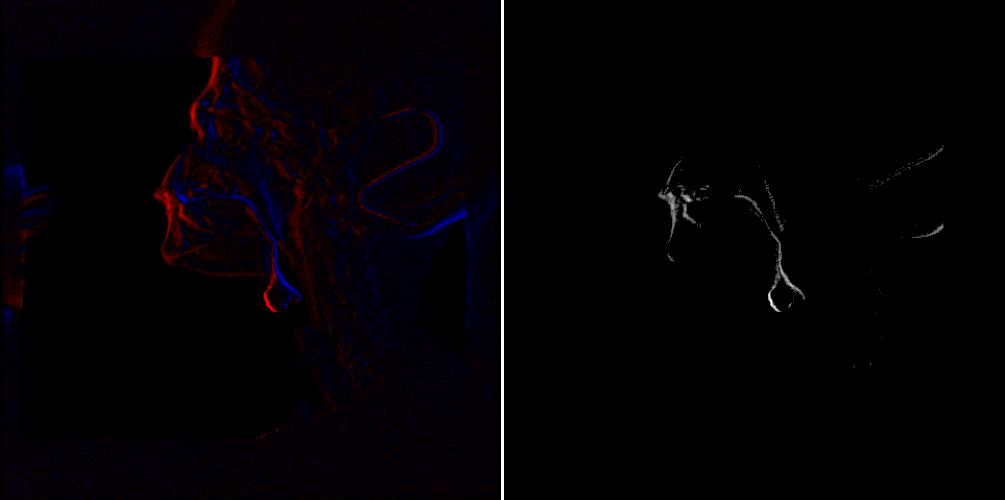
\includegraphics[width=0.8\textwidth]{figures/3_2.png}
    \caption{双边滤波降噪}
    \label{fig:3_3_双边滤波}
\end{figure}

\subsubsection{形态学操作降噪}\label{sec:3_3_2}

在接下来的步骤中,我们需提取图像的轮廓。而获取轮廓的方法所需的输入应为二进制黑白位图。因此,需要将上述操作后得到的灰阶图像进行二值处理。在此过程中,难免会产生一些新的噪点,为此,在二值化操作完成后,还须再实施一轮针对二进制黑白位图的降噪处理。

本研究选用形态学操作的一些基本方法来进行降噪。所涉及的运算包括:腐蚀、膨胀、开运算以及闭运算。以下是膨胀变换和腐蚀变换的描述:
\begin{itemize}
    \item 膨胀变换(Serra, 198蚀和膨胀的定2\cite{serra1982image}):考虑一个区域 $R$ 和一个邻域 $N$。根据定义,用 $N$ 对 $R$ 进行二元扩张得到的网格点集合 $D$ 是与 $R$ 相交的 $N$ 的平移中心的位置,这个集合用 $D=R \oplus N$ 表示。换言之:$D=\{x \in R |(N+x) \cap R \neq \emptyset\}$。
    \item 腐蚀变换(Serra, 1982\cite{serra1982image}):根据定义,用 $N$ 对 $R$ 进行二元侵蚀得到的网格点集合 $E$ 是包括在 $R$ 中的 $N$ 的平移中心的位置,这个集合用$E=R \ominus N$表示。换言之:$E=\{x \in R |(N+x) \subset R\}$。
\end{itemize}
简单来说,使用腐蚀操作得到的结果为原始图像的子集;而使用膨胀操作得到的结果为原始图像的超集。我们可以循环使用这两种操作。若先使用腐蚀操作,后使用膨胀操作,则构成形态学操作中的“开运算”,可以用于去除图像中的边缘“毛刺”;反之,若先使用膨胀操作,再使用腐蚀操作,则构成“闭运算”,可以用于填充图像中的微小“空洞”。两种运算均可以在不明显改变主体结构和形态的情况下平滑边缘。

在本研究中,我们通过以下策略进行降噪:
\begin{itemize}
    \item 获取图像中的轮廓,以及每个轮廓所包围的像素数(详见\cref{fig:3_4})
    \item 统计其中的“小轮廓”数量 $t$
    \item 循环执行以下操作,直到小轮廓数量小于等于阈值 $T_1$,或循环次数到达阈值上限 $T_2$
    \subitem 对当前图像执行一次开运算
    \subitem 循环执行以下操作,直到循环次数到达阈值上限 $T_3$:
    \subsubitem 统计当前图像中小轮廓数量 $t^{\prime}$
    \subsubitem 若$t^{\prime} < t$,终止循环
    \subsubitem 执行一次腐蚀运算
    \item 执行膨胀运算。执行次数等于上述循环中腐蚀运算的总执行次数。
\end{itemize}

在本研究中,若一个轮廓包围的像素数量小于包围像素数最多的轮廓的 $20\%$,则我们称其为小轮廓。此外,以上策略中的阈值可以视情况调整,或采用某种自动阈值算法。在本研究中,$T_1=10, T_2=4, T_3=3$。

\cref{fig:3_3_形态学} 展示了降噪结果。从左到右分别为:原始数据帧、取绝对差图像后行双边滤波降噪后的灰度图、二值化后应用形态学降噪的二值图。

\begin{figure}[!htp]
    \centering
    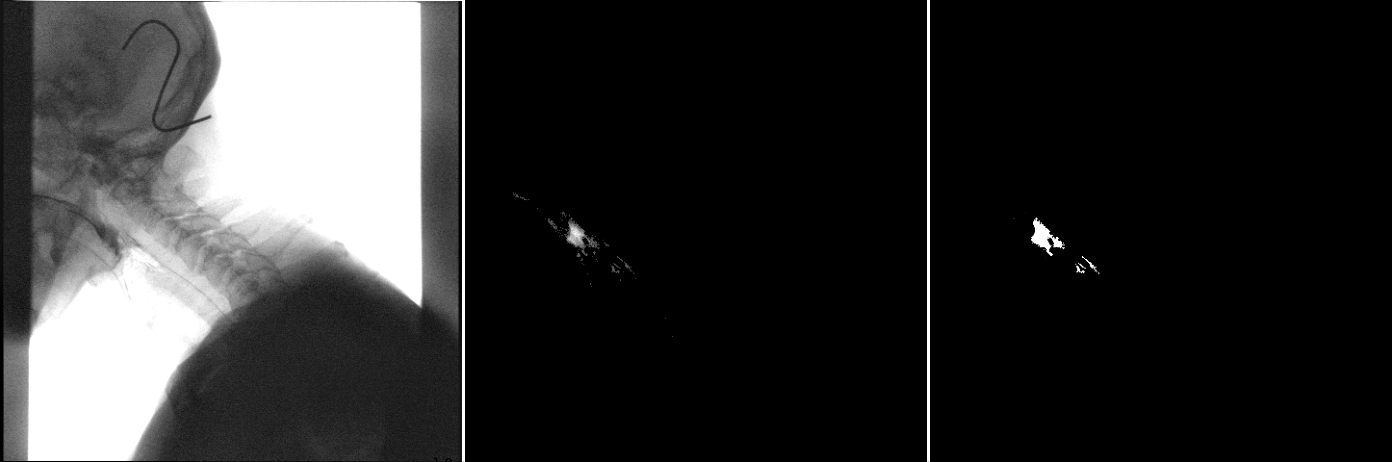
\includegraphics[width=\textwidth]{figures/3_3.png}
    \caption{二值化后行形态学降噪结果}
    \label{fig:3_3_形态学}
\end{figure}

\subsection{获取图像轮廓并过滤}\label{fig:3_4}

\subsubsection{获取图像轮廓}

我们使用了著名的开源模块 OpenCV 中的 findContours() 方法来获取图像轮廓。该方法为Suzuki等人\cite{suzuki1985topological}的研究的C++实现。

算法流程简要概括如下:

\begin{enumerate}
    \item 将输入的二值图像看作是一个二维矩阵,Suzuki算法从左上角开始逐行扫描,直至发现一个像素值为255的点,并以此为始点开始查找轮廓。
    \item 使用一种名为 MOORE邻域 的方法进行逐边追踪。MOORE邻域 由8个像素按固定顺序组成(自左上角起顺时针排列),在跟踪过程中,算法依循此顺序挑选下一个潜在的点位。
    \item 算法会通过对比前一点与找到的后继点,按步建立一个代表轮廓的数据结构。同时,算法还会检测值为255的点的底部是否存在值为0的点,以判断该轮廓是否为内轮廓。
    \item 当算法回到起始发现的像素点,便视为完成了当前轮廓的查找。接着,返回原矩阵,继续自左至右,自上而下地寻找下一个潜在点位。
    \item 算法将持续执行,直至遍历整幅图像并锁定所有轮廓为止。
\end{enumerate}

该算法返回一个由所有轮廓点组成的列表,以及层次结构信息(从树结构表示)。层次结构包括每个轮廓的索引,表示哪一个轮廓是谁的子轮廓、父轮廓和同级轮廓。

\begin{figure}[!htp]
    \centering
    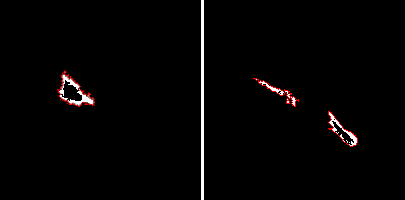
\includegraphics[width=0.8\textwidth]{figures/3_4.png}
    \caption{使用Suzuki算法获取图像轮廓}
    \label{fig:3_4_获取轮廓}
\end{figure}

\subsubsection{获取轮廓包围的像素数}

在\cref{sec:3_3_2} 中,我们多次在图像中寻找所有轮廓,且还需要获取每个轮廓包围的像素数量。因此,我们需要一个高效的从轮廓中统计出面积的算法。在本研究中,我们通过格林公式(Green's Formula)来完成这个任务。格林公式源自数学家乔治·格林(George Green)在1828年发表的一篇有关电磁学的研究报告\cite{green2014}。格林公式是向量微积分领域的一个重要定理,描述了一个平面区域内的曲线积分与区域内的面积的关系。这个定理被广泛应用于包括物理、工程和计算机科学在内的其他领域。尽管它最初的应用针对的是电磁学领域的问题,但格林公式及其各种拓展形式已成为数学和物理学的基础工具。具体来说,可以通过以下公式计算轮廓的面积$S$:
\begin{equation}
    S = 0.5 * |\sum_{i=0}^{n-1}(x_i y_{i+1} - x_{i+1} y_i)|,
\end{equation}

其中,$n$ 为轮廓点的数量,$(x_i, y_i)$ 代表轮廓的第 $i$ 个点。特别的,当 $i=n-1$ 时,$x_{i+1}$ 和 $y_{i+1}$ 指向第一个点($x_0$ 和 $y_0$)。需要注意的是,该方法应用在存在自交点的轮廓上时会得到错误的结果。

\subsection{获取本底值蒙版}

经过以上操作后,我们成功从绝对差图像中过滤噪点,并取得代表钡餐的轮廓。现在,我们需要从轮廓获取轮廓所包围的像素点的集合,而非数量。我们使用泛洪填充算法(Flood Fill Algorithm)来完成这个任务。

该算法首先会寻找任意一个轮廓区域内的像素点。对于凸包,其重心一定在轮廓区域内,因此该问题可以简化为寻找重心。对于一个给定的代表轮廓的二维点集 $P$,其重心计算公式为:
\begin{equation}
    (centroid_x, centroid_y) = (\frac{\sum_{i=0}^{n}x_i}{n},\frac{\sum_{i=0}^{n}y_i}{n}) 
\end{equation}
对于其它形状的轮廓,需要使用其它方法来获取起始像素点。一般会尝试获取轮廓最左边和最上边的点,随后逐行扫描,直到找到满足轮廓之内的点,作为起始点。

接下来,算法会从起始点向四个相邻的像素点展开。如果目标像素点尚未填充颜色并且与起始像素点的颜色相近(在二值图中即为寻找黑色的像素点),该算法会为目标像素点填充颜色。算法会以同样的方式继续向外扩展,并不断填充相邻像素点,直到达到轮廓边界。当所有与初始像素点相邻的区域都已被填充后,泛洪填充算法完成工作。

\begin{figure}[!htp]
    \centering
    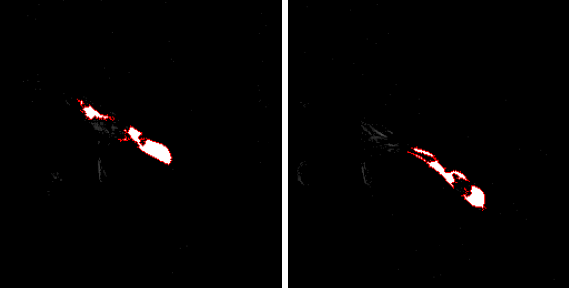
\includegraphics[width=0.8\textwidth]{figures/3_5.png}
    \caption{使用泛洪法填充轮廓}
    \label{fig:3_5_泛洪}
\end{figure}

对于以上操作结果获得的黑白蒙版,将其中每个白色像素的值替换为该像素在当前帧和上一帧中的值中的最小值,作为当前帧本底值。本底值的意义在于记录某像素点在成为钡餐区域之前,其所对应的人体器官或组织在图像中的灰度值。在最终逐帧逐像素标记钡餐浓度时,应根据此本底值做出修正。

\subsection{结果}

\cref{fig:3_结果} 展示了两组经过上述操作后得到的钡餐区域和本底值标注。这两组数据中,钡餐分别位于受试者的口部和喉部。其中,黑色部分代表非钡餐区域。需要注意的是非黑色部分:其亮度越高,代表本底值越低(而非钡餐浓度越高)。

\begin{figure}[!htp]
    \centering
    \begin{subfigure}{\textwidth}
        \centering
        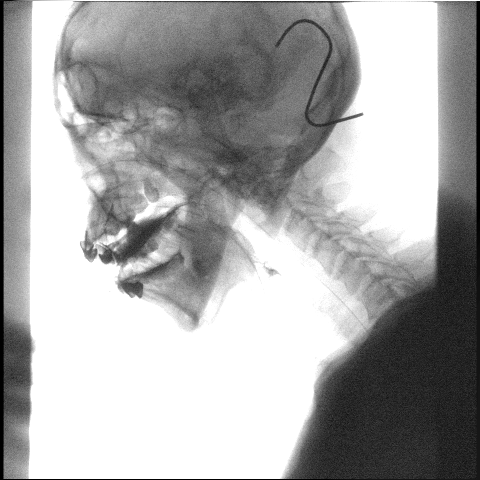
\includegraphics[width=0.4\textwidth]{figures/3611.png}
        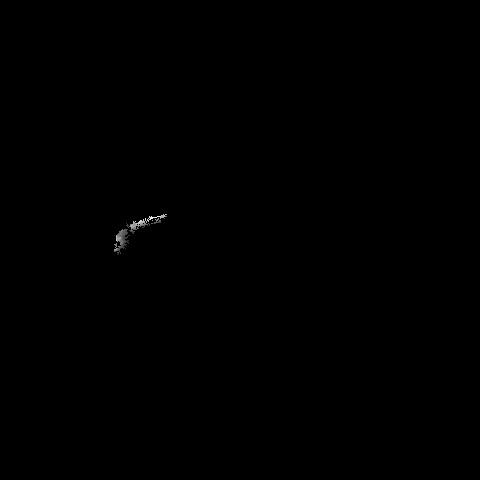
\includegraphics[width=0.4\textwidth]{figures/3612.png}
        \caption{口部}
    \end{subfigure}
    
    \begin{subfigure}{\textwidth}
        \centering
        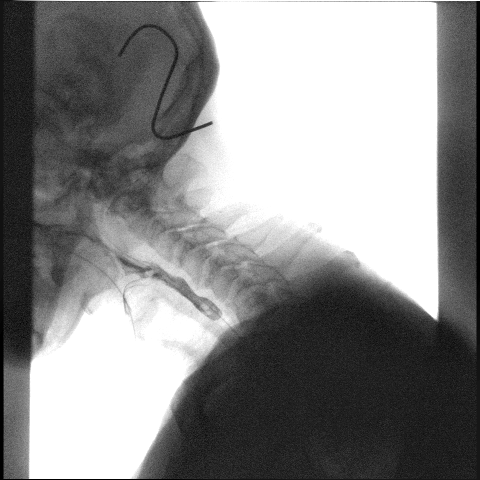
\includegraphics[width=0.4\textwidth]{figures/3621.png}
        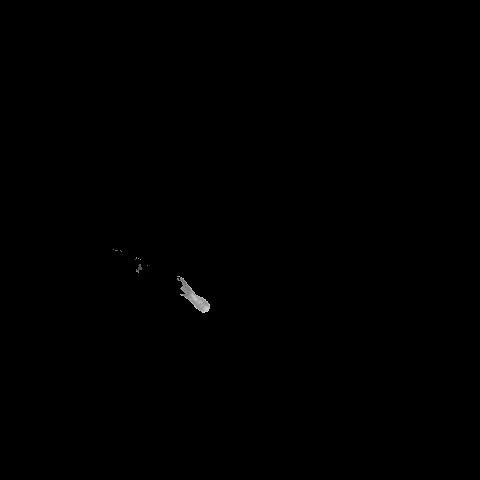
\includegraphics[width=0.4\textwidth]{figures/3622.png}
        \caption{喉部}
    \end{subfigure}
    \caption{钡餐区域和本底值标注}
    \label{fig:3_结果}
\end{figure}

可见,经过上述处理后所得到的结果较为精确。对于口部的数据帧,算法成功地将钡餐从像素值相近的牙齿区域中区分开来;而在喉部数据帧的应用上,算法准确标记出迅速穿越喉咙进入胃部的钡餐,同时也不漏掉附着在喉部的残留钡餐。

\subsection{本章小结}

本章应用多种图像处理算法,提取视频数据中每一帧图像里的钡餐区域及其本底值。操作流程如下:对相邻帧图像求差值,得到待处理图像;对图像进行去噪处理;使用算法获取图像轮廓及每个轮廓所包围的像素数;循环运用腐蚀和膨胀算法筛选并剔除小轮廓以实现进一步去噪;对上述步骤得到的钡餐区域进行本底值标注,生成最终蒙版。